\documentclass[12pt]{report}

\usepackage{amsmath,amsfonts,amssymb,mathtools}
\usepackage{physics,siunitx}
% \usepackage{feynmf}
\usepackage{graphicx,subfig,caption}
\usepackage[hidelinks]{hyperref}

\usepackage[backend=biber,
maxnames=2, style=phys,
articletitle=true,biblabel=brackets,
chaptertitle=false,pageranges=false,
urldate=iso8601,
]
{biblatex}

\addbibresource{references.bib}


\usepackage{abstract}
\usepackage[titletoc,page]{appendix}

\usepackage{titlesec}
\titleformat{\chapter}[display]   
{\normalfont\huge\bfseries}{\chaptertitlename\ \thechapter}{20pt}{\Huge}   
\titlespacing*{\chapter}{0pt}{0pt}{10pt}

\oddsidemargin=0in
\evensidemargin=0in
\textwidth=6.25in
\headsep=0pt
\headheight=0pt
\topmargin=0in
\textheight=9in

\usepackage[T1]{fontenc}
\usepackage[utf8]{inputenc}
\usepackage[swedish,english]{babel}

\setlength{\parindent}{0em}
\setlength{\parskip}{1em}


\begin{document}

\title{AM36}

\author{
    \begin{tabular}{c@{\hskip 1cm}c}
        Yue Jiao         & Mattias Jönsson \\
        \texttt{911024-7799} & \texttt{940425-0673}\\
        \texttt{yj@kth.se} & \texttt{matjon4@kth.se}
    \end{tabular}
    \vspace{0.5cm}\\
    SH1012 Modern Physics
}

\date{April 14, 2016 \\
Revised version}

\maketitle

\tableofcontents

\chapter{Introduction}
In 1934 Maire Curie died due to the high radiation dose she had received during her years of research with radioactive materials. Today we better know the dangers of radiation exposure and it is therefore of great interest to know how much of a given material is needed in order to stop the radiation. Stopping the radiation from $\alpha$ or $\beta$ sources is fairly simple since these decay particles are charged and therefore are affected by electromagnetic force. A charged particle traveling through a material will affect the surrounding particles and therefore loose energy as it travels.

Stopping the radiation from $\gamma$ sources is not as easy since the $\gamma$ particles have zero charge. In order to safely shield a $\gamma$ source a heavy material such as lead is usually needed. Using lighter material will result in unreasonable dimensions for the shielding material. The thickness of the material is also dependent on the energy of the $\gamma$ radiation, since higher energy $\gamma$ particles will penetrate further into the material.

This paper will investigate how the radiation intensity is dependent on the energy of the $\gamma$ particles, the material and the thickness of the material. Two materials, lead and tin, will be used in the experiments and the primary goal is to determine the stopping coefficient for each material and energy.

\chapter{Theory}

\section{Matter interactions}
In this experiment photons may interact with matter by either Compton scattering or photo-electric absorption. The two interactions are similar and involves a photon interacting with a electron. In photo-electric absorption the electron will absorb all of the energy from the photon, causing the photon to disappear and the electron will be released from the its atom. In Compton scattering only parts of the energy from the photon will be transferred to the electron causing the electron to be released from its atom. This time, however, the photon will not disappear.

There is a third way photons may interact called pair-production. If a photon has sufficient energy, more than $1.022MeV$, an electron and a positron may spontaneously be created and the photon is destroyed. The energies in this experiment are generally to low for pair-production to occur and therefore the effects of pair-production will be neglected.

\section{Scintillator detector}
In order to detect a particle, it must interact with matter inside the detector. Building a radiation detector therefore requires that the radiation can stop inside the detector, however it is also required to filter any unwanted background radiation. To full fill both these needs a scintillator detector have a so-called window to filter away any unwanted radiation and a so-called scintillator that captures the wanted radiation. When measuring $\gamma$ radiation, the window is a piece of metal that blocks $\alpha$ and $\beta$ radiation form entering the detector, but is thin enough to let $\gamma$ radiation through. When a $\gamma$ photon have passed through the window it will enter the scintillator.

Inside the scintillator, the $\gamma$ photon may interact with an atom, either by Compton scattering or by photo-electric absorption. This will cause the atom to release an electron that will travel through the scintillator material. During it’s travel, the electron will excite an atom in it’s surrounding, which then will cause it to de-excite and release low energy photons.

The released photons will then enter another part of the detector, the so-called Photo-Multiplier-Tube (PMT). Inside the PMT the photons will smash into a metal plate and by the photo electric effect an electron will be released. The electron will then be accelerated by a strong electric field forcing it to smash into another metal plate, causing multiple electrons to be released. This process is repeated multiple times until a measurable amount of electrons is generated. Using electronics it is then possible to detect both the number of detected particles and the energy of these particles.

A calibration of the detector is needed to get a reliable result from the energy measurement. This is required since the exact strength of the electric field inside the detector is unknown. Using multiple samples of radioactive sources with known radiation peaks it is possible to interpolate a polynomial $P : B \leftarrow E$, where $B$ is the bins and $E$ is the energies. The polynomial may then be used to convert from a given bin $B_i \in B$ to the
equivalent energy $E_i \in E$.

\section{Gamma spectrum}
\begin{figure}[ht]
    \centering
    
    \subfloat[Cs-137 spectrum]{
        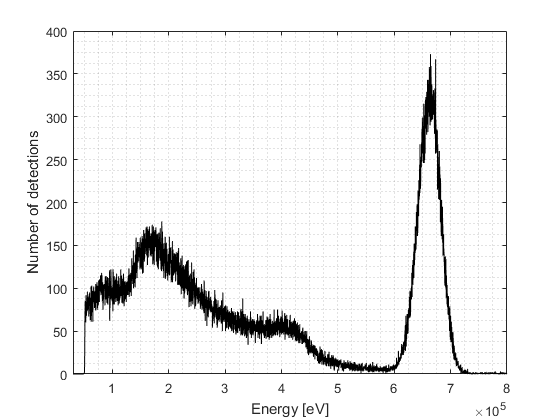
\includegraphics[width=0.8\textwidth]{cs137spectrum}
        \label{figure:cs137spectrum}
    }
    
    \subfloat[Co-60 spectrum]{
        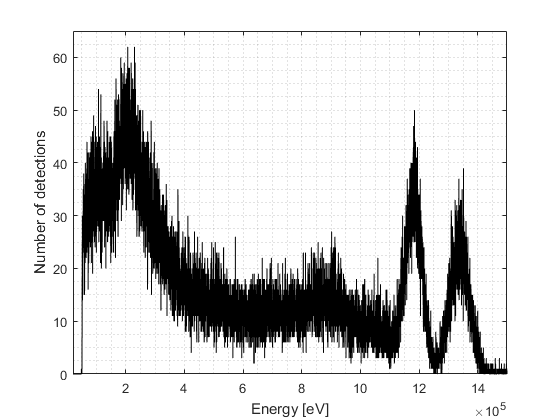
\includegraphics[width=0.8\textwidth]{co60spectrum}
        \label{figure:co60spectrum}
    }
    
    \caption{Two $\gamma$ spectra showing the characteristic properties. The first peaks are X-rays and the following peaks are decay detections. The continuous part of the spectra is Compton scattering detections.}
    
\end{figure}
A typical $\gamma$ spectrum is semi-discrete with sharp peaks and a continuous distribution (see figure 2.1). The sharp peaks originates from X-rays and from photo-electric absorption of radiation from the measured isotope, whereas the continuous distribution originates from Compton scattering of the radiation.

The low energy peaks in a $\gamma$ spectrum are detections of X-rays that were created when the gamma photons hit a dense material. This dense material could be the sample itself or lead surrounding the sample during the measurements.

The high energy peaks are photo-electric absorption detections of $\gamma$ photons sent out from the material. Since the energy of a given photon is determined only by the decay process, all $\gamma$ photons sent out from a radioactive material will have discrete energies. The measurement of these photons will then result in a discrete spectrum since all of the $\gamma$ photons’ energy is contained in the detector. The high energy peak seen in figure \ref{figure:cs137spectrum} corresponds to when Barium-137m de-excite, which releases a photon energy of $611.7keV$ \cite{nudatCs}. Barium-137m is present in the sample since it is a daughter of Cesium-137. The two high energy peaks seen in figure \ref{figure:co60spectrum} correspond to when Nickle-60m de-excite in a two step process first releasing a $1173.2keV$ photon and then releasing a $1332.5keV$ photon \cite{nudatCo}. Nickel-60m is present in the sample since it is a daughter of Cobalt-60.

Between the X-ray peak and the characteristic $\gamma$ peak there is a smaller peak. This peak is due to backscattering inside the protective lead box. When a photon hit the bottom of the lead box it may backscatter and in the process lose some of its energy. The photon will then travel in the opposite direction and may be detected with reduced energy.

\pagebreak
The continuous energy are measurements from Compton scattering of the $\gamma$ photons. Since the energy transferred to the electron during Compton scattering is dependent on the collision angle, the spectrum measured is continuous. The angle dependence also implies that there is a maximum energy for the continuous spectrum. Therefore the maximum energy of the Compton scattering occurs when the photon backscatters. In figure \ref{figure:cs137spectrum} the Compton scattering spectrum ends at approximately $450keV$ . In figure \ref{figure:co60spectrum} the Compton scattering spectrum ends around $1 MeV$. The edge is less distinct than for Cesium-137, which is because there are two photon energies and therefore there must
be two ends to the Compton scattering spectrum.

\section{Statistical distribution for decay}
The probability for a given decay event is $p$. Given that there will be multiple events occurring during a time-limited measurement this implies that the decay will be Poisson distributed $Po(z)$. The standard deviation $\sigma$ may therefore be expressed as $\sigma = \sqrt{z}$,which is the square root of the number of detections.

\chapter{Experimental setup}
\begin{table}[ht]
    \centering
    \begin{tabular}{|l|l|}
     \hline
        Protective lead box     & Sample of Am-241 enclosed in plastic \\ \hline
        Scintillator detector   & Sample of Co-60 enclosed in plastic \\ \hline
        Dial caliper            & Sample of Cs-137 enclosed in plastic \\ \hline
        Lead plates             & Tin plates \\ \hline
    \end{tabular}
    \caption{The material used in the experiment.}
    \label{tab:material}
\end{table}

The equipment used in this experiment is listed in table \ref{tab:material}.

All measurements in the following experiments were recorded using the program Tukan with the stop-criteria set to $60s$ live time. This means that each measurement was in real time run $60s$ plus the dead time, which is the time it took for the detector to reset and getting ready for the next measurement. A lower energy threshold was set in Tukan in order to reduce high background noise.

The spectrum of each radioactive sample was measured in the detector without any lead or tin plates blocking the detector. From the spectra the bin of characteristic peaks were recorded and compared to reference values \cite{nudat} and the data was fitted using a polynomial. The polynomial was used to calibrate the bins to their corresponding energy.

The thickness of the lead and the tin plates was measured using the dial caliper. The spectrum of each radioactive sample was then measured with $0$, $1$, $2$, $4$, $8$ and $16$ plates covering the sample. From each peak in the spectra a Region of Interest (RoI) was assigned, where each RoI spanned an energy interval so the peak was inside that interval. The number of detections for each RoI was the recorded. A non-linear curve fitting algorithm was used to fit the data to the model
\begin{equation}
    I = I_0 e^{-\mu d},
\end{equation}
where $d$ is the distance the photons travel through the material.

\chapter{Results}

\section{Calibration}
Given the three radioactive samples there is a total of four possible data points\footnote{There are two characteristic peaks for Cobalt-60.}, however only three were used. The Americium-241 is not included when fitting the polynomial (see the discussion for a motivation). The data points used for the calibration is listed in \ref{tab:cal}.

\begin{table}[ht]
    \centering
    \begin{tabular}{|c|c|c|}
    \hline
        Sample  &    Energy $[keV]$  &    Bin \\ \hline
        Cs-137  &    661.7           &    3628.28 \\ \hline
        Co-60   &    1173.2          &    6228.73 \\ \hline
        Co-60   &    1332.5          &    7059.96 \\ \hline
    \end{tabular}
    \caption{The data points used to calibrate the detector.}
    \label{tab:cal}
\end{table}

The resulting polynomial fit is
\begin{equation}
    E(b) = -82.25 + 0.211b - 1.5\cdot10^{-6}b^2.
\end{equation}

\section{Thicknesses of plates}
\begin{table}[ht]
    \centering
    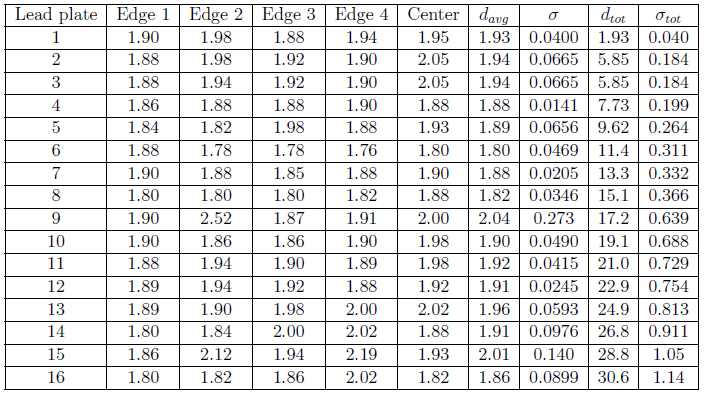
\includegraphics[width=1\textwidth]{t1}
    \caption{Thickness of the lead plates with corresponding mean thickness and standard deviation.}
    \label{tab:t1}
\end{table}

The thicknesses of the lead plates are presented in table \ref{tab:t1} and the thickness of the thinner lead plates are presented in table \ref{tab:t2}.

\begin{table}[ht]
    \centering
    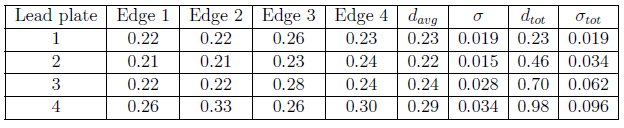
\includegraphics[width=1\textwidth]{t2}
    \caption{Thickness of the thinner lead plates with corresponding mean thickness and standard deviation.}
    \label{tab:t2}
\end{table}

The thicknesses of tin plates do not vary since they are hard enough to resist being bent. All tin plates are therefore assumed to have the thickness $2.0mm$, with a standard deviation of the smallest measurable distance using the caliper $\sigma = 0.1mm$.

\section{Parameter fit}
In the table below the parameter fits are presented with the corresponding value taken from NIST \cite{nist}. Diagrams for the parameter fits are presented in figure \ref{figure:cs137} for Cesium-137, figure \ref{figure:co6011732} for Cobalt-60 $1173.2keV$ and figure \ref{figure:co6013325} for Cobalt-60 $1332.5keV$ . Americium-241 was removed from the parameter fit since the lower energy threshold was set high enough to interfere with the measurement of the peak. The parameters when travelling through lead are presented in table \ref{tab:ldata} and the parameters when travelling through tin are presented in table \ref{tab:tdata}.

\begin{table}[ht]
    \centering
    \begin{tabular}{|c|c|c|c|}
    \hline
        Peak energy $[keV]$ & Calculated $\mu [mm^{-1}]$ for lead   & $\chi^2_{red}$    & Reference $\mu [mm^{-1}]$ \\ \hline
        $661.7$               & $0.111 \pm 0.002$                   & $2.18$            & $0.142$\\ \hline
        $1173.2$              & $0.0641 \pm 0.0007$                 & $0.826$           & $0.0806$\\ \hline
        $1332.5$              & $0.0610 \pm 0.0007$                 & $0.916$           & $0.0667$\\ \hline
    \end{tabular}
    \caption{Parameters for when travelling through lead.}
    \label{tab:ldata}
\end{table}

\begin{table}[ht]
    \centering
    \begin{tabular}{|c|c|c|c|}
    \hline
        Peak energy $[keV]$ & Calculated $\mu [mm^{-1}]$ for lead   & $\chi^2_{red}$    & Reference $\mu [mm^{-1}]$ \\ \hline
        $661.7$               & $0.0982 \pm 0.0005$                 & $3.38$            & $0.0591$\\ \hline
        $1173.2$              & $0.0533 \pm 0.0007$                 & $0.228$           & $0.0423$\\ \hline
        $1332.5$              & $0.0562 \pm 0.0008$                 & $0.307$           & $0.0371$\\ \hline
    \end{tabular}
    \caption{Parameters for when travelling through tin.}
    \label{tab:tdata}
\end{table}

\begin{figure}[ht]
    \centering
    
    \subfloat[Cs-137 through lead parameter fit]{
        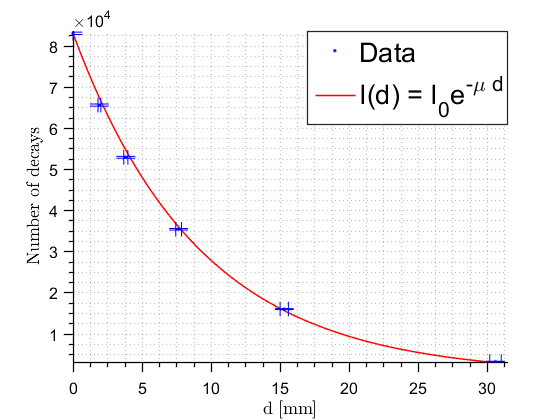
\includegraphics[width=0.8\textwidth]{cs137lead}
    }
    
    \subfloat[Cs-137 through tin parameter fit]{
        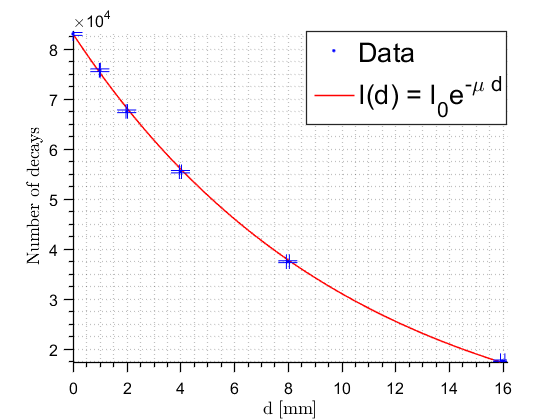
\includegraphics[width=0.8\textwidth]{cs137tin}
    }
    
    \caption{The parameter fits for Cs-137.}
    \label{figure:cs137}
    
\end{figure}

\begin{figure}[ht]
    \centering
    
    \subfloat[Co-60 $1173.2keV$ through lead parameter fit]{
        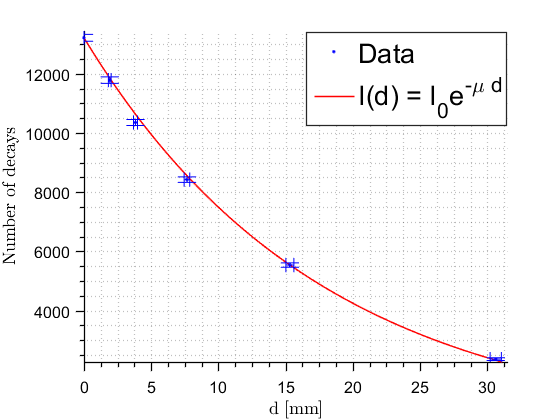
\includegraphics[width=0.8\textwidth]{co60lead11732}
    }
    
    \subfloat[Co-60 $1173.2keV$ through tin parameter fit]{
        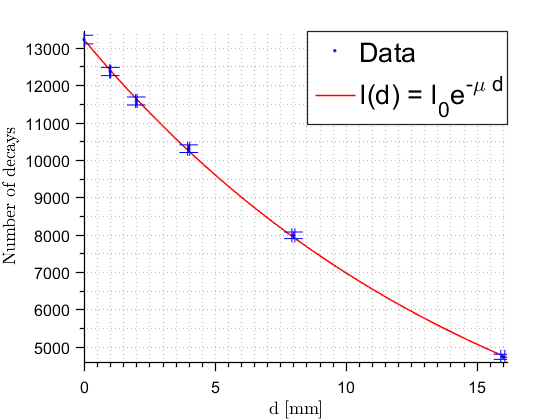
\includegraphics[width=0.8\textwidth]{co60tin11732}
    }
    
    \caption{The parameter fits for Co-60 with $1173.2keV$.}
    \label{figure:co6011732}
    
\end{figure}

\begin{figure}[ht]
    \centering
    
    \subfloat[Co-60 $1332.5keV$ through lead parameter fit]{
        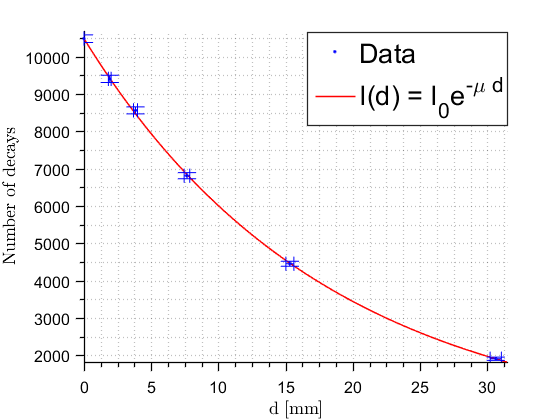
\includegraphics[width=0.8\textwidth]{co60lead13325}
    }
    
    \subfloat[Co-60 $1332.5keV$ through lead parameter fit]{
        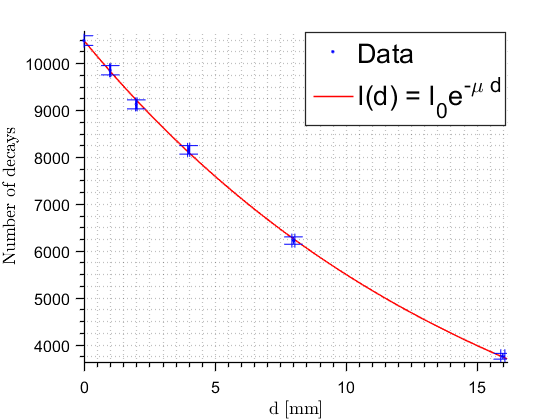
\includegraphics[width=0.8\textwidth]{co60tin13325}
    }
    
    \caption{The parameter fits for Co-60 with $1332.5keV$.}
    \label{figure:co6013325}
\end{figure}

\chapter{Discussion}
\section{Exclusion of Americium-241}
The analog-to-digital-converter used in this experiment had a large low energy noise which caused the dead time to be disproportionally large in comparison to the live time. Therefore the time in order to collect a sufficient data was much larger than the live time since the detector had to reset to so often. In order to prevent the experiment from taking unreasonable time to complete a lower energy threshold was set. It was necessary to set the threshold to a level where it interfered with the measurements of Americium-241. This resulted in inconclusive data and therefore the Americium-241 measurements were removed from this experiment.

\section{Goodness of fit}
In the experiments with Cesium-137, $\chi^2_{red} > 1$ which suggest that the model do not fit the data especially well or that the estimations of the errors are to small. A too small error estimation in the thickness of the plates is probably not the case with the lead plates. A more likely explanation would be a systematical error where a noise signal interferes with the measurements. Another possibility could be that the stack of plates in the tin case was slightly tilted causing the travel distance in the material to be greater than expected. A final explanation would be that the RoI was too large and therefore included data not only coming from the peak, but also data from Compton scattering with the walls of the protective lead box or with the plates themselves.

In the measurements of Cobalt-60 radiation travelling through tin, $\chi^2_{red} < 1$ suggesting that the model is fitting errors. Setting the thickness error to zero for all data points does not significantly improve the $\chi^2_{red}$ values, which suggests that the decay errors are over-estimated. This could be explained by a systematical error where noise interferes with the measurements. This noise could from Compton scattering with the walls of the protective lead box or with the plates themselves.

\newpage
In the measurements with Cobalt-60 and tin, the value of $\mu$ is lower for $1173.2keV$ than it is for $1332.5keV$, which is is not expected. The expected result would be that a lower energy photon is easier to stop and therefore $\mu$ should be higher for higher energies. A possible explanation could be that Compton scattering from the higher energy level has enough energy to be in the measured interval for the lower energy. Since the maximum energy a photon can transfer to an electron through Compton scattering is when the photon backscatters, it is possible to calculate this energy. The detected energy is described by
\begin{equation}
    E_{detected} = E - \frac{c^2}{\frac{1 - \cos{\theta}}{m_e} + \frac{c^2}{E}} = \{Backscatter \implies \theta = -1, E = 1332.5keV\} = 1118 keV.
\end{equation}
Since $1118keV$ is in the interval used in the measurement, backscatter of the higher energy will have interfered with the measurement of $\mu$ for $1173.2keV$.

\section{Comparision the absorption in tin and lead}
From this experiment it is obvious that lead is a better material when trying to stop gamma radiation. The value of $\mu_{lead}/\mu_{tin} = 1.8$ is independent of the energy of the radiation, which possibly could be explained by the fact that $\rho_{lead}/\rho_{tin} = 1.5$. The connection between large values for $\mu$ and $\rho$ is most likely because a material with high $\rho$ will have more particles per volume for the photon to interact with. In a material with high electron density the probability for Compton scattering and photo electric absorption should be higher than in a material with lower electron density. When comparing the electron density the result is
\begin{equation}
    \frac{Z_{lead}n_{lead}}{Z_{tin}n_{tin}} = \frac{Z_{lead}m_{lead}M_{tin}}{Z_{tin}m_{tin}M_{lead}} = \{V_{lead} \approx V_{tin}\} = \frac{Z_{lead}\rho_{lead}M_{tin}}{Z_{tin}\rho_{tin}M_{lead}} \approx 1.5,
\end{equation}
which would explain why lead has a higher $\mu$.

\printbibliography

\end{document}
